\begin{figure}[htbp] \centering
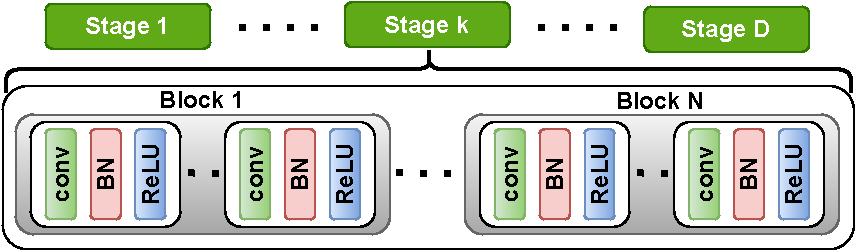
\includegraphics[scale=0.55]{Figures/NetHierarchy}
\vspace{-1em}
\caption{The structure of conventional ResNet-like architectures: %\cite{he2016deep,zagoruyko2016wide,
%xie2017aggregated,huang2017densely,huang2018condensenet,brendel2018approximating}.
Stages comprise Blocks and Blocks comprise multiple repetitions of conv, BN, and ReLU layers. 
%We follow this hierarchy in DeepReDuce in order to reduce the huge search space for ReLU optimization.
%this is the terminology we use to describe how ReLU dropping optimizations are applied.
}
\vspace{-1em}
\label{fig:NetHierarchy}
\end{figure}